\subsubsection{Feature discovery with dashboards and AI agents}
\label{subsubsection:rebuttal_dashboards_feature_discovery}

This section expands on the \textit{Visualization and interpretation} paragraph of \hyperref[subsubsection:latents_evaluation_details]{\ref*{subsubsection:latents_evaluation_details}} and describes how dashboards and AI agents support feature discovery in practice.

\paragraph{Cycling through latents.}
Discovery starts from a dashboard built from a trained model's saved latent activations and the behavioral and environmental variables recorded alongside the neural data; building it requires no retraining. Each view shows one latent: its activation as a function of chosen variables, and its strongest activating episodes alongside behavior. A researcher cycles quickly through latents, one keystroke per latent, viewing each latent's activity as a function of behavioral or environmental variables to judge its potential interpretability. \autoref{figure:rebuttal_dashboards_churchland} and \autoref{figure:rebuttal_dashboards_aeon} show examples of dashboards that can be used in this workflow, for the recordings and models of \hyperref[subsection:churchland_results]{\ref*{subsection:churchland_results}} and \hyperref[subsection:aeon_results]{\ref*{subsection:aeon_results}}. Feature dashboards developed for sparse autoencoders trained on language models are related examples, such as Anthropic's feature browser~\citep{bricken_2023_towards_monosemanticity}\footnote{\url{https://transformer-circuits.pub/2023/monosemantic-features/vis/a1.html}} and Neuronpedia's feature dashboards~\citep{lin_2023_neuronpedia}\footnote{\url{https://docs.neuronpedia.org/sparse-autoencoders/feature-dashboards}}.

\paragraph{Narrowing a feature description.}
When a latent looks promising, the researcher either analyzes it further themselves to narrow the feature description, or hands it off to an AI agent. Narrowing a description means, for example, adding variables to the view, varying one variable while holding another fixed, and inspecting examples in which the latent is active outside the candidate condition or inactive within it. A hand-off consists of the latent, the saved activations and recorded variables, and a short instruction telling the agent what to look for; the agent carries out this follow-up analysis and returns a proposed condition and comparison population for the researcher to review. Final descriptions are scored with the metrics of \hyperref[subsubsection:latents_evaluation_details]{\ref*{subsubsection:latents_evaluation_details}}.

\paragraph{Agent-first screening.}
As an alternative to cycling through latents first, an agent can score every latent against a set of behavioral and environmental conditions, for example by computing \metric{Sel} and \metric{AUROC} for each latent--condition pair, and return ranked candidates. The researcher then opens the highest-ranked latents in the dashboard and proceeds as above.

\paragraph{Time and effort.}
The time and effort required vary with the number of latents, the number of recorded variables, and the structure of the experiment. For the Aeon dataset (\hyperref[subsection:aeon_results]{\ref*{subsection:aeon_results}}), a single researcher did an initial cycle through 100 latents in less than one hour. The work was parallelized: the researcher continued to cycle through latents while handing off promising latents to an agent to explore in more detail, telling the agent what to look for. The \textit{wheel activity} latent (\autoref{fig:aeon_features}) is an example.

\begin{figure}[!htbp]
    \centering
    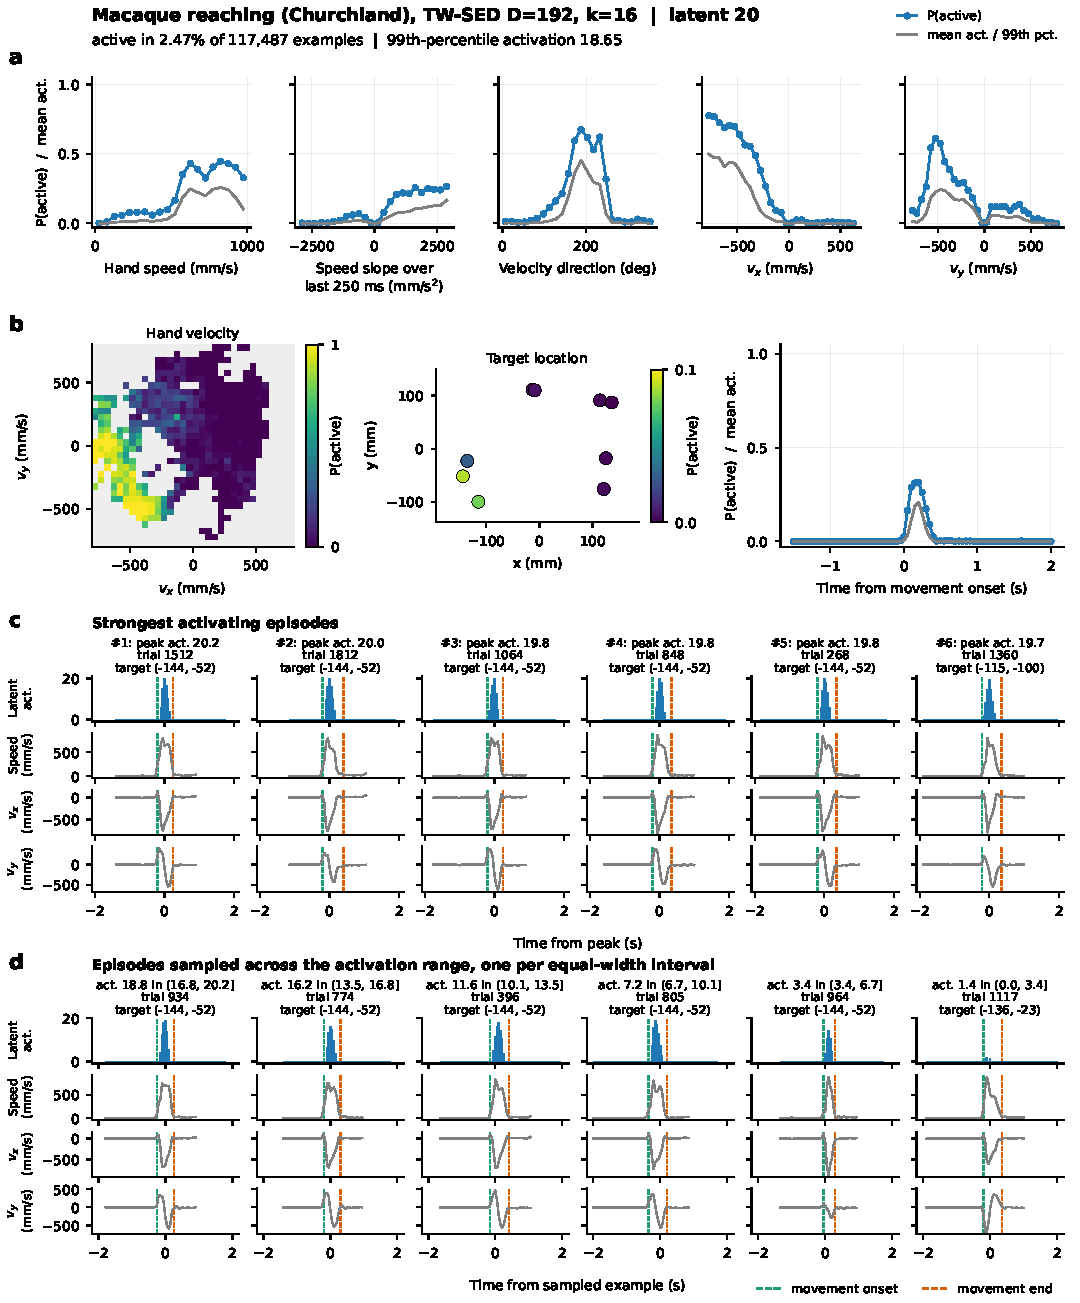
\includegraphics[width=\linewidth]{figures/rebuttal/change07_dashboards/dashboard_churchland_latent20.pdf}
    \caption{\textbf{Example dashboard view for the macaque reaching recording.} One view of a dashboard that can be used in the feature discovery workflow, shown for latent 20 of the $D=192$, $k=16$ model of \hyperref[subsection:churchland_results]{\ref*{subsection:churchland_results}} (the \textit{fast leftward target reach} latent), using the 117,487 windows of the development trials. (\textbf{a}) Activation as a function of five kinematic variables: activation probability (blue) and mean activation as a fraction of the latent's 99th-percentile positive activation (gray), per bin. (\textbf{b}) Activation probability by hand velocity (light gray: fewer than 10 windows) and by target location, each with its own color scale, and activation as a function of time from movement onset. (\textbf{c}) The six strongest activating episodes, each from a different trial, above hand speed and velocity; dashed lines mark movement onset and end. The dashboard steps from one latent to the next with the arrow keys.}
    \label{figure:rebuttal_dashboards_churchland}
\end{figure}

\begin{figure}[!htbp]
    \centering
    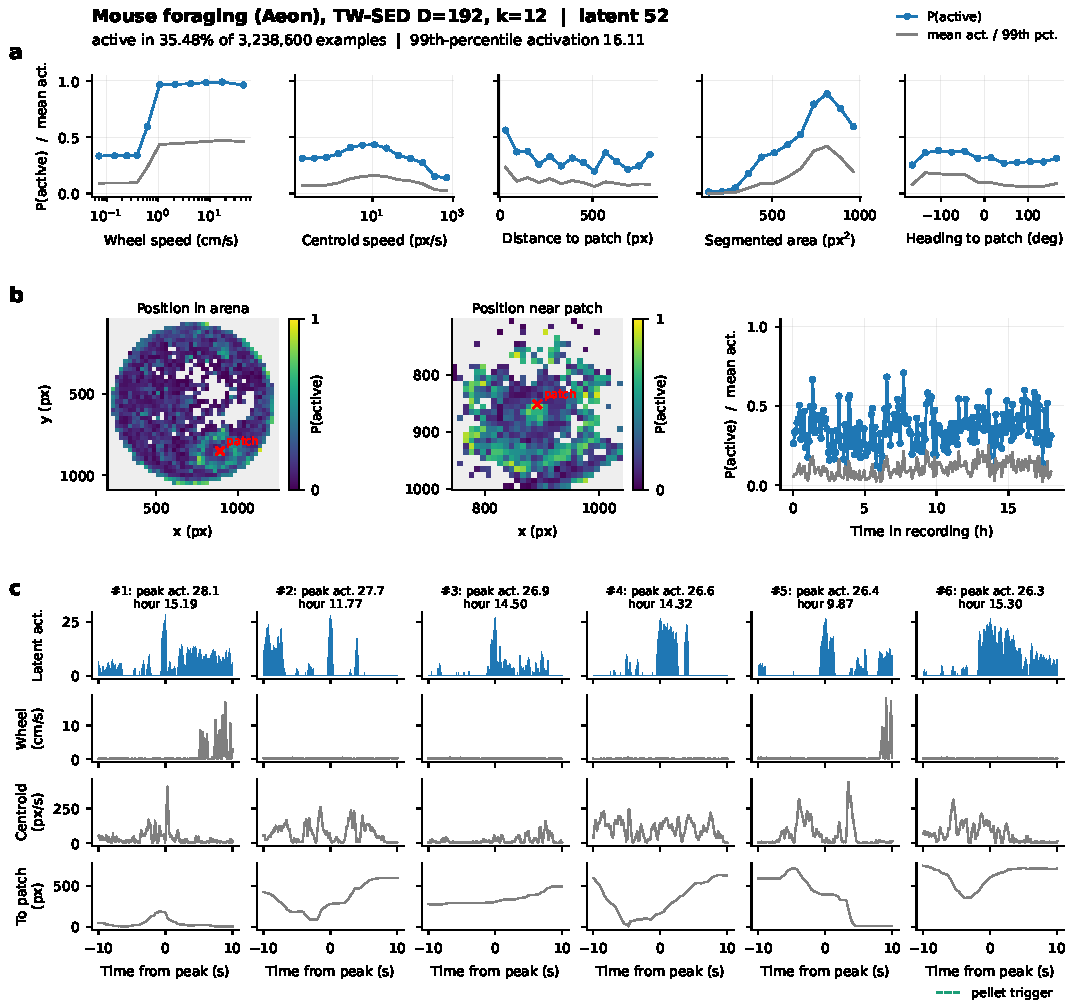
\includegraphics[width=\linewidth]{figures/rebuttal/change07_dashboards/dashboard_aeon_latent52.pdf}
    \caption{\textbf{Example dashboard view for the mouse foraging recording.} One view of a dashboard that can be used in the feature discovery workflow, shown for latent 52 of the $D=192$, $k=12$ model of \hyperref[subsection:aeon_results]{\ref*{subsection:aeon_results}} (the \textit{wheel activity} latent), using all 3,238,600 windows. (\textbf{a}) Activation as a function of wheel speed, centroid speed, distance to the patch, segmented image area, and movement heading relative to the patch: activation probability (blue) and mean activation as a fraction of the latent's 99th-percentile positive activation (gray), per bin. (\textbf{b}) Activation probability by position in the arena and near the patch (red cross; light gray: fewer than 50 windows), and activation over the 18-hour recording in 5-minute bins. (\textbf{c}) The six strongest activating episodes, at least 20 s apart, above wheel speed, centroid speed, and distance to the patch, for 10 s either side of each peak.}
    \label{figure:rebuttal_dashboards_aeon}
\end{figure}
